\documentclass{article}

\usepackage[francais]{babel}
\usepackage[T1]{fontenc}
\usepackage[utf8]{inputenc}
\usepackage{eurosym}
\usepackage{array}
\usepackage{graphicx}
\usepackage{fancyhdr}
\usepackage{verbatim}
\usepackage{enumerate}

\pagestyle{fancy}
\fancyhf{}
\rhead{Issidi}
\lhead{Rapport de 1\iere{} soutenance}
\rfoot{Page \thepage}


\title{Rapport de 1\iere{} soutenance\\
		Issidi\\
		Debil.OS();}
\author{Jérémy \bsc{Beuvry}\\
		Julien \bsc{Boulicaut}\\
		Clément \bsc{Finck}\\
		Sébastien \bsc{Fleury}}

\begin{document}
\maketitle
\centerline{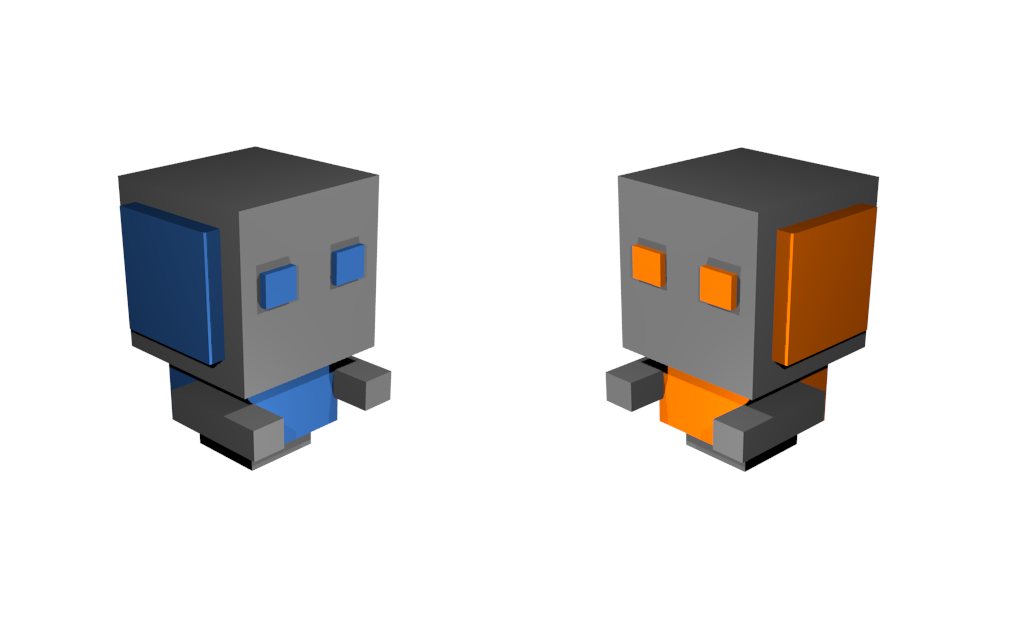
\includegraphics[scale=0.5]{rf.png}}
\newpage
\tableofcontents
\newpage

\section{Introduction}
Notre groupe, les ''Debil.OS();'' est fier de vous présenter son premier raport de soutenance du projet Issidi.
\newline\newline Ce projet prend la forme d'un jeu de tir à la troisième personne dans un univers post apocalyptique.  Les principal mécaniques du gameplay et l'univers sont rappeler 

\centerline{
\includegraphics[scale=0.2]{latex_sa_pue.png}}
\centerline{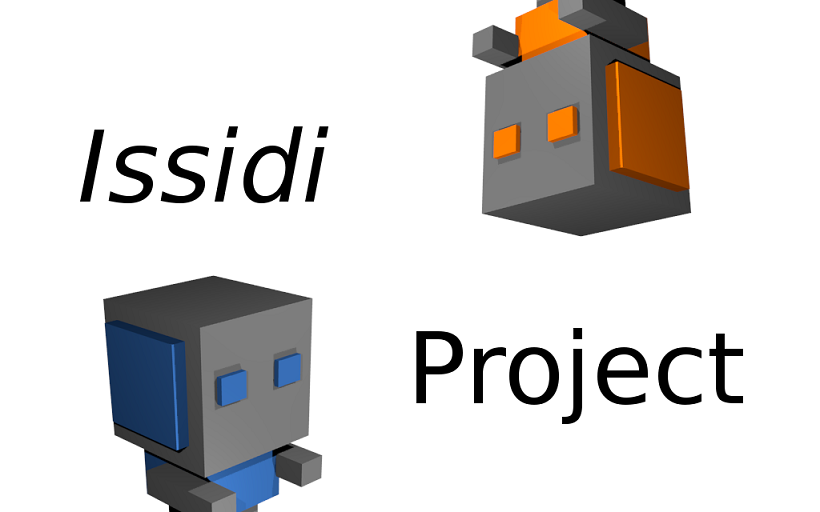
\includegraphics[scale=0.5]{styler.png}}


\section{Rappel du cahier des charges}

\subsection{Scenario}
Dans un monde ravagé par la guerre tous les hommes sont morts ou enterrés, mais pas nécessairement dans cet ordre.
En effet, les radiations résultant du grand bombardement ont rendu la surface de la Terre létale pour l'humanité telle que nous 
la connaissons. 
Les rares survivants sont contraints de se terrer dans des bunkers antiatomiques pour pouvoir espérer qu'il y ait un jour lointain un retour possible à la surface. En attendant, seuls leurs drônes peuvent se risquer au-dehors pour récupérer des matériaux quand il en reste.
Très vite, les ressources se font rares et des luttes éclatent peu à peu.
Incarnez un pilote de drone de combat en récupérant un maximum de matériaux nécessaires à la survie des camarades de votre abri et en déjouant les assauts des autres
pillards assoiffés de métal. 
Vous représenterez l'ultime rempart entre la vie et la mort pour vos frères, alors, laisserez-vous l'humanité sombrer sans agir ?

\newpage\subsection{Mécanique de jeu}
\centerline{
\includegraphics[scale=0.2]{latex_sa_pue.png}}

 Issidi est un jeu de tir à la troisème personne(aussi appelé \emph{Third Person Shooter}),
qui sera créé avec le moteur de jeu Unity3d, édition personnelle.

Pour les déplacement en plus de ceux classique vous pourrez également esquiver à l'aide de petit saut rapide vers 
l'avant ou encore utiliser des doubles sauts qui permettront aussi d'atteindre certaines zones qui auraient
 été inaccessibles sinon.

Plusieurs armes seront disponibles pour varier le gameplay et permettre à tous les types de joueurs de prendre
 un maximum de plaisir. Que vous adorez tout faire exploser avec une lance rocket, ou un rythme plus rapide avec 
un fusil d'assaut, même les fans de corps à corps pourront même s'essayer à la vivisection laser sur robots. 
ainsi que différentes cartes.

Le mode multijoueurs mettra en scène les batailles sanglantes entre pillards de ressources dont un seul 
sortira vainqueur, ou pas !


\subsection{Physique}
Cette section sera dédiée à la gestion des interactions des différents élements avec la gravité.
Ainsi que la gestion de tous les types de collisions: joueur/terrain,projectile/joueur, projectile/terrain ( pour à terme, permettre d'avoir un
environnement partiellement destructible). Parmi les interactions on notera en particulier la possibilité de marcher sur 
les murs et le plafond, via une rotation du vecteur gravité, qui constituera l'une des principales mécaniques du jeu.


\subsection{Particules}
Afin d'améliorer la beauté de ce projet, l'ajout de particules est indispensable!
On pourra par exemple faire apparaître la trainée des différents projectiles, afin de montrer leurs
trajectoires. Ou encore de dynamiser l'action et d'égailler les décors.

\subsection{Arme}
Un robot sans défense n'a aucun intérêt s'il ne possède rien lui permettant d'occire ses ennemis, 
il doit donc disposer d'un arsenal suffisant. Il sera donc nécessaire de créer plusieurs armes
afin d'ajouter une profondeur au gameplay.


\subsection{Interface}
Afin de rendre le jeu plus convivial, celui-ci doit posséder 
une interface composée de plusieurs menus. Celle-ci 
permettra notamment de naviguer dans les options du jeu, de
 lancer une partie en mode solo, ainsi que de choisir les
 paramètres des parties du mode multijoueur.

\newpage\subsection{Site Web}
Le site web nous permettra de montrer l'avancement de notre projet.Il contiendra une description du projet, des images de celui-ci, ainsi
que des liens permettant d'avoir un accès rapide aux sources du projet.

\centerline{
\includegraphics[scale=0.2]{latex_sa_pue.png}}
\centerline{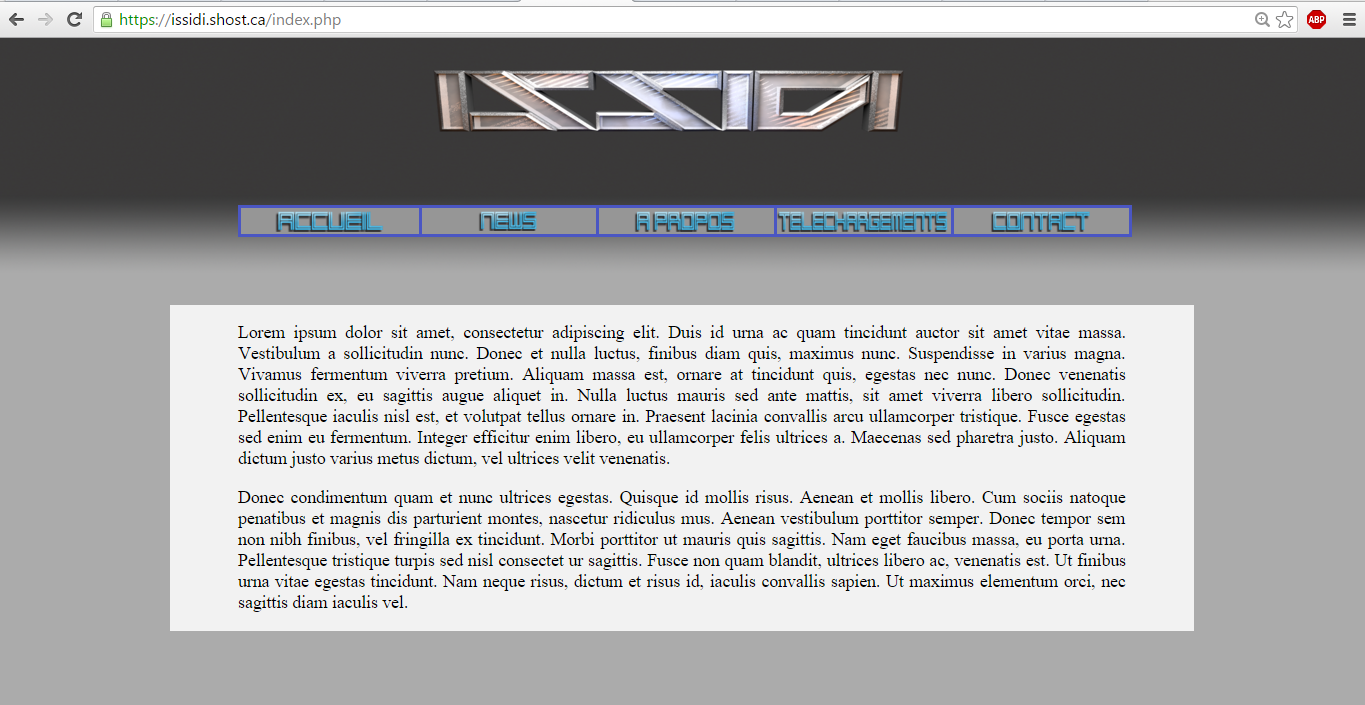
\includegraphics[scale=0.4]{screen_site1v2.png}}
\centerline{
\includegraphics[scale=0.2]{latex_sa_pue.png}}
\centerline{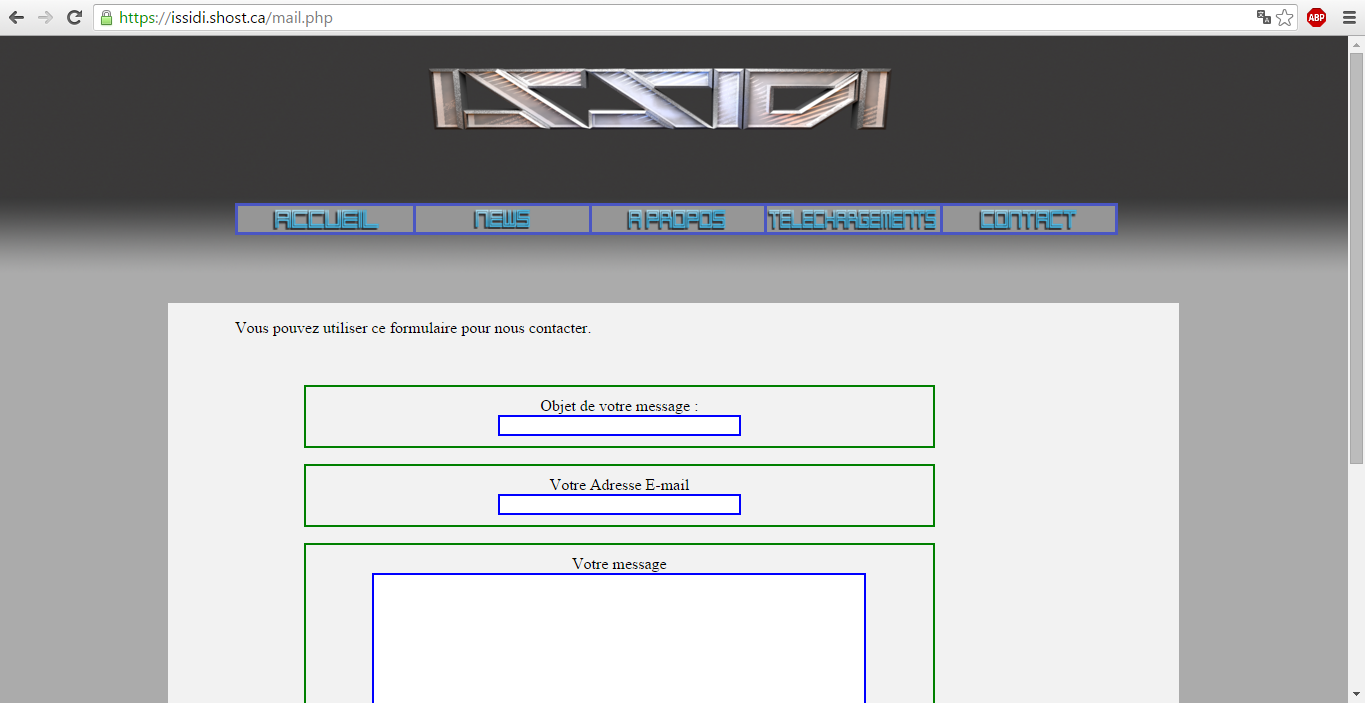
\includegraphics[scale=0.4]{screen_site2v2.png}}


\section{Répartition des tâches}

\begin{tabular}{|c|c|c|c|c|}
\hline
			&	Jérémy		&	Julien		&	Clément		&	Sébastien	\\ \hline
Site Web	&				& $\bigotimes$	& 				& $\bigcirc$	\\ \hline
Physique	&				&				& $\bigcirc$	& $\bigotimes$	\\ \hline
Multijoueur	& $\bigotimes$	& $\bigcirc$	&				& 				\\ \hline
Animation	&				& $\bigotimes$	& $\bigcirc$	&				\\ \hline
IA			& 				& $\bigotimes$	& $\bigotimes$	&				\\ \hline
Particules	& $\bigcirc$	& 				&				& $\bigotimes$	\\ \hline
Personnage	& $\bigotimes$	&				& 				& $\bigcirc$	\\ \hline
Arme		& $\bigcirc$	&				&				& $\bigotimes$	\\ \hline
Son			&				& $\bigcirc$	& $\bigotimes$	&				\\ \hline
Modèles		& $\bigotimes$	&				& $\bigotimes$	&				\\ \hline
Interfaces	& 				& $\bigcirc$	& $\bigotimes$	&				\\ \hline
\end{tabular}

Légende:\\
$\bigotimes$ : s'occupe de\\
$\bigcirc$ : aide

\section{Planning}
\subsection{1\iere{} soutenance}
\begin{tabular}{|c|c|}
\hline
			&	Premiere Soutenance	\\ \hline
Site Web	&	XX		\\ \hline
Physique	&	X		\\ \hline
Multijoueur	&			\\ \hline
Animation	&			\\ \hline
IA	        &			\\ \hline
Particules	&	X		\\ \hline
Personnage	&	XX		\\ \hline
Arme		&	X		\\ \hline
Son			&			\\ \hline
Modèles		&	XX		\\ \hline
interface	&	X	    \\ \hline
\end{tabular}


Légende :\\
X : partie commencée\\
XX : partie à moitié faite\\
XXX : partie finie

\subsection{Éléments effectués}
\subsubsection{Interface}
\begin{itemize}
\item[+] Ajout du menu principal
\item[+] Ajout d'un menu pause
\item[+] création de la barre de vie
\end{itemize}

\subsubsection{Physique}
\begin{itemize}
\item[+] Ajout d'une boite de collision pour le personnage, afin de lui permettre d'évoluer dans le monde
\item[+] Modification de la gravité en fonction de son axe
\item[+] Changement de l'axe du personnage lors de l'appui sur \emph{E}.
\end{itemize}

\subsubsection{Particules}
\begin{itemize}
\item[+] Les balles sont suivit de particules, représentant la traînée.
\end{itemize}

\subsubsection{Personnage}
\begin{itemize}
\item[+] Possibilité de se déplacer
\item[+] Échange possible de son axe de mouvement
\item[+] Le personnage peut dasher (accélérer brutalement), impossibilité de changer de direction lors du dash
\item[+] Double sauts possible
\item[+] Caméra à la 3\ieme{} personne
\end{itemize}

\subsubsection{Arme}

\begin{figure}[h]
\centerline{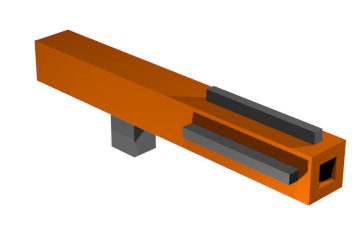
\includegraphics[scale=0.5]{rocket_launcher.png}}
\caption{Un lance roquette}
\centerline{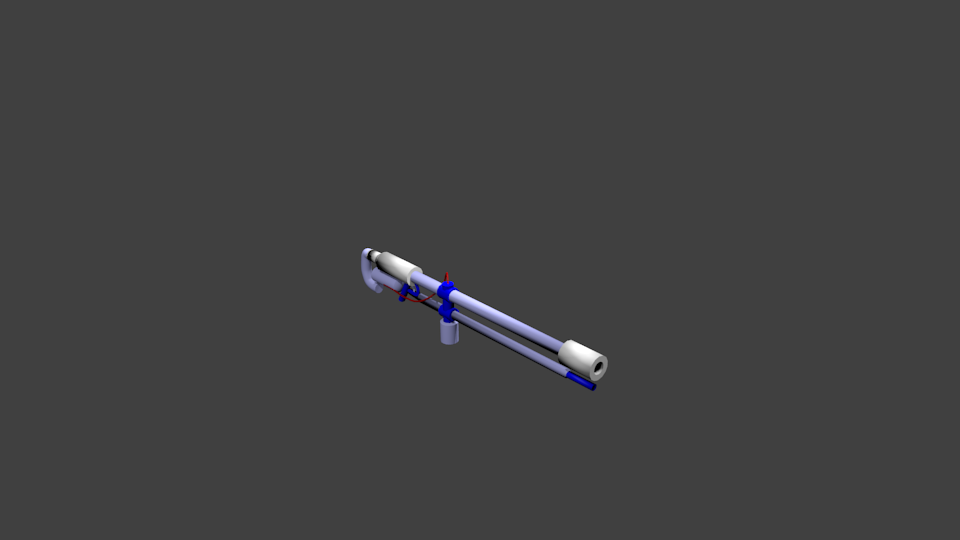
\includegraphics[scale=0.5]{ff.png}}
\caption{Un lance flamme}
\end{figure}

\subsubsection{Créations des modèles}
\begin{itemize}
\item[+] Personnages
\item[+] Armes variées
\item[+] Point de respawn
\item[+] Tourelles
\item[+] Araignée suicidaire
\item[+] Map prédécoupé
\end{itemize}

\subsubsection{Interface}
Menu pricipal:
\newline Un menu principal étant indispensable , nous en avons rajouter un très sobre en attendant d'avoir
affiné notre charte graphique. Le menu principal permettra de charger les différents mode de jeu, d éditer les options
et de quitter le jeu.
\newline\newline Menu pause:
\newline Ce menu permet en mode solo de mettre en pause le jeu (\begin {verbatim}Time.timescale=0f
\end{verbatim}) ou de revenir au menu principal. En multijoueur le temps ne sera pas arrête.Quand au 
design ,comme pour le menu principal, nous avons choisit de rester simple. Néanmoins les dimensions
elles, sont variable et s'adapte a la résolution de l'écran.
\newline\newlineBarre Barre de vie:  
\newlineUne barre de vie étant indispensable dans un TPS, nous en avons creer une de manière très discrète en haut à gauche de l'écran.
Celle-ci permettra de monitorer la vie de notre personnage ayant un bref aperçu du maximum de vie possible ainsi que de la vie que nous possédons.
La barre de vie est composée, donc, de 2 éléments distincts, un en fond qui indique le montant maximum de vie et un en premier plan qui indique la vie effective de notre personnage.

\subsection {Particules}
Si les particules ont un effet paillettes, elles sont ici représentatives, 
par exemple de la portée d'une de nos armes, un lance-flamme. Le système de 
particules intégré à Unity étant complet, on peut très facilement grâce des 
textures (notamment ici, le feu) rendre à peu près n'importe quel effet désiré. 
On contrôlera la taille à l'aide d'une courbe "sise over lifetime". Le lance-flammes 
était un peu particulier par rapport aux balles, il nécessite un script de plus 
pour contrôler son system de particules et ainsi être actif uniquement sur demande.

\begin{verbatim}
if (Input.GetButton("Fire1"))
    {
         em_mod.enabled = true;
    }
    else
    {
         em_mod.enabled = false;
    }
\end{verbatim}

em\_mod étant l'émission module du particle system.

\centerline{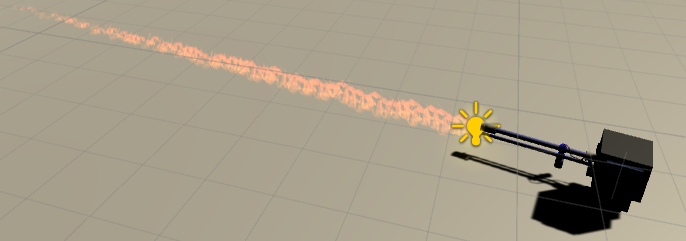
\includegraphics[scale=1.0]{flamethrower.png}}

\subsection {Physique}

Le centre de notre jeu étant le fait de pouvoir marcher les murs et plus 
généralement changer la gravité, cet aspect devait impérativement être 
réalisé le plus tôt possible dans la conception afin de développer tous 
les autres autours de celui-ci. Pour ce faire, on va regarder dans toutes 
les directions si un mur est disponible à l'aide d'un raycast, on va garder 
en mémoire tous ceux ayant une distance inférieure à une portée maximum.
On gardera le mur le plus proche pour nouvelle direction de gravité.
Le vrai défi de ce script était-ce celui-ci détecte bien où s'accrocher.

\begin{verbatim}
foreach (KeyValuePair<Vector3,Deplacement.Direction> Vec in Asso)
        {
            if (Vec.Value != d.sens)
            {
                RaycastHit R;
                Physics.Raycast(t.position, Vec.Key, out R);
                if (R.collider != null)
                { 
				//Notre verifiation de la distance
\end{verbatim}
				
Avec "Asso" un dictionaire permettant d'associer un vecteur et une direction de gravité.

\begin{verbatim}
Dictionary<Vector3, Deplacement.Direction> Asso = new Dictionary<Vector3, Deplacement.Direction>()
    {{Vector3.forward, Deplacement.Direction.mZ},
     {Vector3.back, Deplacement.Direction.Z},
     {Vector3.up, Deplacement.Direction.mY},
     {Vector3.down, Deplacement.Direction.Y},
     {Vector3.left, Deplacement.Direction.X},
     {Vector3.right, Deplacement.Direction.mX},
    };
\end{verbatim}
		
(Ici on dessine les diferents axes possibles)

\centerline{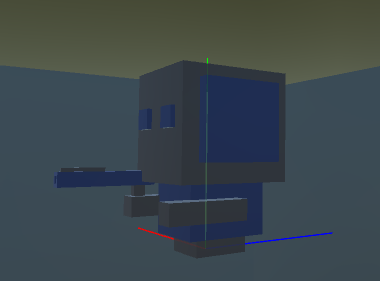
\includegraphics[scale=1.0]{test_gravity.png}}


\subsection {Tir et Arme}

Cette partie fut une des premières à être complétée, mais rendu rapidement 
non exploitable a cause du changement de gravité, les différentes rotations 
n'étant plus les mêmes par rapport aux vecteurs "World".
Pour le suivit de l'arme par la caméra, nous utilisons un point de pivot 
artificiel. Le modèle 3d étant centré sur sa scnene, son point de pivot 
se retrouve au centre du modèle, ce qui n'est pas l'endroit désiré. Le 
modèle est donc enfant d'un empty. Le système principal des armes, le fait 
de tirer utilise lui aussi un empty, les balles partiront celui-ci, légèrement 
devant le modèle pour éviter une collision immédiate avec le collider du 
personnage. Les balles sont instanciés, permettant de modifier une référence 
et de toutes les modifier par la même occasion.

\begin{verbatim}
        Vector3 shootSpeed = new Vector3(Speed, 0, 0);
        GameObject bullet = Instantiate(template);
        bullet.transform.position = transform.position;
        Rigidbody body = bullet.GetComponent<Rigidbody>();
        body.AddForce(transform.forward * 500);
\end{verbatim}
		
Uniquement deux armes sont disponibles pour le moment, un fusil basique et un 
lance-flamme. Le fusil basique utilise des balles visibles alors que le lance-flammes 
lui utilisera des balles invisibles et un système de particules pour montrer l'endroit visé.

\centerline{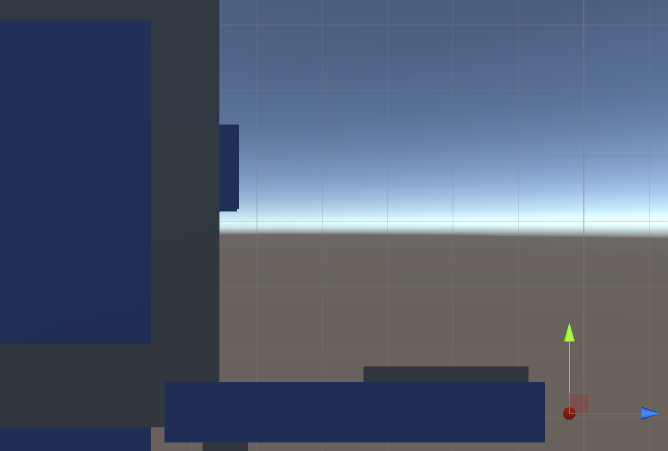
\includegraphics[scale=1.0]{empty.png}}


\section{Présentation des éléments effectués individuellement}
\subsection {Personnage}
\subsubsection{Déplacement}
De part la nature de notre interface, où nous povons changé d'axe à tout moment,
il nous est impossible d'utiliser les prefabs d'Unity, c'est pourquoi il a fallu
recoder les déplacements.
Ainsi, afin de pouvoir nous déplacer correctement quelque soit l'axe, nous avons utilisés :
\begin{verbatim}
Vector3 transform.forward
Vector3 transform.right
\end{verbatim}
qui désigne respectivement les vecteurs directionnels : frontal et droit, appartenant tous les deux au transform
Ainsi, il ne nous reste plus qu'à récupérer les événements utilisateur (l'appui des touches) grâce à :
\begin{verbatim}
Input.GetAxis("Horizontal")//Déplacement gauche droite
Input.GetAxis("Vertical")//Mouvement avancer/reculer
\end{verbatim}

afin de pouvoir déplacer facilement notre personnage, quelque soit l'axe sur lequel il se trouve.
ce qui donne donc :
\begin{verbatim}
Vector3 vitesse_deplacement = Input.GetAxis("Horizontal") * transform.right +
							  Input.GetAxis("Vertical") * tranform.forward;
\end{verbatim}

\subsubsection{Physique du personnage} \label{physique_personnage}
Afin d'ajouter la présence d'une gravité pour notre personnage, qui change si l'on change d'axe,
il a fallut désactiver la gravité implémentée de base dans Unity. En effet, comme le montre le schéma
ci-dessous :

\centerline{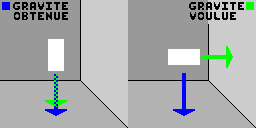
\includegraphics[scale=1.5]{explication_gravite.png}}

lors d'une rotation du personnage (quand l'on marche sur le mur par example), la gravité reste toujours la
même, c'est-à-dire sur l'axe des y, or nous voudrions que celle-ci s'adapte en fonction du joueur.
C'est pourquoi nous avons décidé de refaire une gravité simple, qui est exprimé comme cela :
\begin{verbatim}
Vector3 vitesse_gravite_personnage = gravity * direction * time;
\end{verbatim}
Le fait que nous calculons uniquement la vitesse, en non la nouvelle position du joueur
s'explique par le fait que lors de l'ajout d'une boîte de collision :
\begin{verbatim}
CollisionBox
\end{verbatim}
le moteur physique d'Unity ne fonctionne pas, si l'on déplace directement
le personnage d'une position à une autre. Il à donc été choisi de non plus modifier la position
du joueur, mais sa vitesse, en réinitialisant la vitesse du personnage sur son axe de déplacement,
et en ajoutant sa vitesse-gravite-personnage et sa vitesse-déplacement, ce qui donne donc :
\begin{verbatim}
//rénitialisation de la velocité sur les axes de déplacement
collision_box.velocity = new Vector3(collision_box.velocity.x * Mathf.Abs(direction.x),
                                     collision_box.velocity.y * Mathf.Abs(direction.y),
                                     collision_box.velocity.z * Mathf.Abs(direction.z),)
collision_box.velocity += vitesse_gravite_personnage + vitesse_deplacement;
\end{verbatim}
Ainsi, nous pouvons avoir un personnage qui se déplace et possédant une physique.

\subsubsection{Double saut}
Le double saut est une des mécaniques secondaires de notre jeu, indispensable
à un jeu de plateforme.
nous avons décidé lors d'un saut de ne pas pouvoir déplacer le personnage,
afin d'obliger les joueurs à utiliser le changement de direction
plutôt que le saut.

\subsubsection{Dash}
Le Dash, une des mécaniques de ce jeu les plus simples à implémenter :
Il ne suffit que d'augmenter la vitesse du personnage temporairement,
tout en empêchant de refaire cette action si elle est en cours.
De plus, nous avons choisis de bloquer la caméra durant le dash qui empêche le changement
de direction du personnage, qui est la contrepartie à la vitesse soudainement augmentée.


\subsection{Modèles}
\subsubsection{Description}
Les modèles sont une partie importante d'un projet, c'est pour cela qu'ils ne doivent pas être négligés.
Nous avons décidé d'avoir des modèles cubiques, pour plusieures raisons :
Tout d'abord, il est très simples de le faire, et ne demande pas de grandes compétences en modélisation.
Ensuite, cela nous évite de devoir prendre dans les assets standard de Unity, et donc d'avoir un projet personnalisé.
Dernièrement, cela nous permet d'avoir des modèles qui seront plus simples à animer.
\newline\newline La map:
\newline Les modèles des maps doivent prévoir le fait que le décor serat destructible a l'avenir. Pour ce fait nous avons creer une map qui est subdivisée en de nombreuses unités independetes.
Celles-ci permettront donc la destruction partielle de la map sans pour autant qu'une tire dans un mur n'entraine pas la destruction intégrale dudit mur.
De plus UNITY ne permetant pas, selon nos connaissances, de détruire partiellement un objet ou une entité mais ne peut gérer que la destruction de l'entité entière.
Il nous a donc paru évident que la map doit être resegmentée en une multitude d'objets afin de pouvoir prévenir la destruction de celle-ci.
\newline\newline Le lance flamme:
\newline Nous possédons deux modèles d'armes dont un lance-flamme.
Celui-ci a ete dessine pour représenter au mieux la réalité et aussi pour s'intégrer au mieux à l'univers du jeu.


\subsubsection{Exemples}
\centerline{
\includegraphics[scale=0.2]{latex_sa_pue.png}}





\subsection{Site Web}
	\subsubsection{Intérêt du site}
 Le site internet doit à terme compléter le projet. Il permettra entre autre de suivre la progression d'issidi  via la rubrique des news et  de regrouper de nombreuses informations relatives au background et aux différents membres du groupe. Enfin, il servira également de sauvegarde pour les membres de notre groupe qui pourront y trouver les rapports de soutenance , des captures d'écrans et même, à terme, un lien pour télécharger le jeu.
 
	\subsubsection{Structure du site}
	Le site se compose de 5 grandes sections : 
1) L’accueil : Cette rubrique
 représente simplement la page d’accueil du site et contient une description d'Issidi et de son univers. 
 2) Les news : Cette rubrique recense les avancées réalisées dans le cadre du projet
(soutenances, première apparition du réseau...)
 3) A propos : cette rubrique est
 divisée en quatre parties correspondant chacune à la présentation d’un des membres du groupe. 
 4) Téléchargements : cette rubrique contiendra les sources du jeu, le cahier des charges et les rapports de soutenance et autres liens utiles. 
 5)Lien «contacts» : dans cette rubrique, il est possible de nous envoyer un mail ce qui s'avérera sans doute très utile aux supps  de l'année prochaine qui se poseront des questions sur le projet.
 
	\subsubsection{Réalisation du site}
	Avancement:
	A ce jour le site web est en ligne à l'adresse : Issidi.shost.ca . la structure générale 
est terminée et seuls le contenu et le design	pourront être soumis à des changements.
	Choix de l'hébergeur :
	Nous avons choisi shost pour plusieurs raisons; la première étant qu'il est gratuit, bien entendu. Et s'il existe effectivement une myriade d'autres d'hébergeurs gratuits, beaucoup imposent des  pubs sur votre site pour se rémunérer. Ce n'est pas le cas de Shost.
De plus, avec shost, nous avons une adresse simple et facile à retenir.Il faut bien reconnaître 
que Issidi.shost.ca se retient bien mieux que Issidi.hebergeurtropbiensuperpratique.com.
Enfin le petit plus de shost  c'est son service technique qui répond très rapidement (moins de 12h) et en français.

 

	
\section{Planning de la 2\ieme{} soutenance}
\begin{tabular}{|c|c|}
\hline
			& Deuxieme soutenance\\ \hline
Site Web	& XXX	\\ \hline
Physique	& XXX	\\ \hline
Multijoueur	& XX	\\ \hline
Animation	& X		\\ \hline
IA	        & X		\\ \hline
Particules	& XX	\\ \hline
Personnage	& XXX	\\ \hline
Arme		& XX	\\ \hline
Son			& X		\\ \hline
Modèles		& XX	\\ \hline
interface	& XX	\\ \hline
\end{tabular}

\section{Récit de la réalisation}
\subsection{Issidi.shost.ca}
Dés la réalisation du site à la rentrée de janvier, nous avons rencontré nos premières difficultés et expérimenté nos premières joies en les surmontant. 
\newline  En effet, si la confection de la structure du site (HTML,PHP) s'est déroulée sans souci particulier, la vraie mise en forme en CSS a elle, en revanche, présenté de nombreux challenges.
\newline	Le premier étant plutôt courant lorsque qu'on fait du design: que faire ? Quelles couleurs utiliser , quelle formes choisir ? etc...
Après plusieurs concertations avec les membres du groupe nous sommes arrivés au design actuel qui nous convient à tous.
\newline	Dans un premier temps, persuadés  (à tort) de connaître suffisamment CSS pour avancer sans aide, nous avons vite compris que nous perdions énormément de temps en appliquant des méthodes désuètes, par exemple en tentant de réaliser le bandeau avec les propriétés des tableaux. Bien Heureusement nous avons découvert l'inline-block qui permet d'avoir des boites contenant du texte et de  taille modulable. La deuxième partie de la solution est venu du TP en c shrap sur les classes; il a permis une utilisation intelligente des div class et des Id qui a conduit à une factorisation de la page de style, la rendant ainsi plus claire et plus simple à modifier.
\newline\newline
Conclusion:
\newline Ainsi nous avons réappris l'importance de définir les spécifications de ce que l'on veut faire avant de se lancer tête baissée dans la réalisation. Et aussi qu'il ne faut pas se surestimer et constamment chercher si de nouvelles méthodes existent. Et le cas échéant, ne pas se contenter de copier-coller la partie de code qui fait ce que l'on veut mais prendre le temps de bien comprendre comment ça marche pour gagner du temps à l'avenir.

\subsection{Déplacement}
La réalisation des déplacements était un grand moment de solitude, surtout lors de la création de fonctionnalités,
qui après une lecture de la documentation Unity, permettait de compacter le code, mais surtout de devoir réécrire
totalement la fonctionnalité.
Malgré tout, c'est aussi une joie de voir qu'Unity possède une quantité énorme de fonctionnalités
afin de faciliter la création de choses différentes que d'habitude

\subsection{Armes et particules}
J'ai été très agréablement surpris de trouver un systeme de particules complet mais aussi très semblables à de nombreux autres logiciels. Cela m'a permi d'être putôt rapide à la conception des effet de particules. Le raycast de Unity est très puissant et permet d'avoir la distance entre le point de départ et d'impact, facilitant énormement la verification pour le changement de gravité.

La gestion des angles sous Unity est.. étrange. Il est impossible d'avoir des angles negatifs, ce qui pose problème pour l'orientation de l'arme. Le raycast de Unity ne génère pas forcement un point d'impact, ce qui est logique mais à provoqué plusieurs fois des erreurs, maintenant corrigées.

\subsection {La map}
Après des essayes assez nombreux, il se trouve que presegmenter un bâtiment en de nombreux objets, cubes dans notre cas, surcharge la mémoire RAM de l'ordinateur sur lequel tourne notre projet.
C'est pourquoi il me faut trouver un autre moyen de rendre destructibles les maps que je crerai a l'avenir sans utiliser cette méthode.

\subsection {La barre de vie}
La barre de vie meme si fonctionnelle reste tres sobre du fait que je n'ai pas reussi a changer sa couleur generale.
En effet je n'ai reussi a changer que la couleur d'un pixel de la barre de vie qui s'instensie avec la couleur par default.
Malgre cela la barre de vie reste tres fonctionnelle et simple.

\subsection{Conclusion}

\end{document}

